\documentclass[10pt]{article}
	\usepackage[utf8]{inputenc}
	\usepackage[onehalfspacing]{setspace}
	\usepackage{enumitem}
	\usepackage{varwidth}
  \usepackage{graphicx}
  \usepackage{listings}
  \usepackage{color}
	\usepackage{geometry}
  \usepackage{lscape}
  \usepackage{float}
  \usepackage{textcomp} % \texttrademark
  \usepackage{multicol}
	\PassOptionsToPackage{hyphens}{url}\usepackage{hyperref}
	\usepackage{hyperref}
  \setlist{nosep, after=\vspace{\baselineskip}}
  \setlength{\columnseprule}{0pt}
  \graphicspath{ {images/} }
  \lstset{language=python,
  frame=single,
  basicstyle=\footnotesize\ttfamily,
  captionpos=b,
  tabsize=2,
  }

\begin{document}

%%%%%%%%%%%%%%%%%%%%%%%%%%%%%%%%%%% /TITLE PAGE %%%%%%%%%%%%%%%%%%%%%%%%%%%%%%%%
\begin{titlepage}
	\centering
  % \vspace{1cm}
  {\scshape\Large USI\par}
	{\scshape\Large Theory of Computation\par}
	\vspace{4.5cm}
  {\huge\bfseries SAT Lab\par}\vspace{0.5cm}
	{\large\bfseries Practical Homework 2\par}
  \vspace{2.5cm}
  {\Large\bfseries Sudoku Solver\par}\vspace{0.5cm}
	\vspace{6cm}
	{\Large Andrea Frachini, Davide Bucher, Lorenzo Spoleti, Milo Wroblewski, Samuele Bischof\par}

\end{titlepage}
%%%%%%%%%%%%%%%%%%%%%%%%%%%%%%%%%%% TITLE PAGE/ %%%%%%%%%%%%%%%%%%%%%%%%%%%%%%%%

\section*{Application}
The web application is bundled with Electron.
The application can be installed on MacOS, but requires python
to be installed.\par\vspace{0.5cm}
The application can be found here on \href{https://github.com/samuelebischof-ch/sudoku-sat}{GitHub}.

\begin{figure}[H]
  \centering
  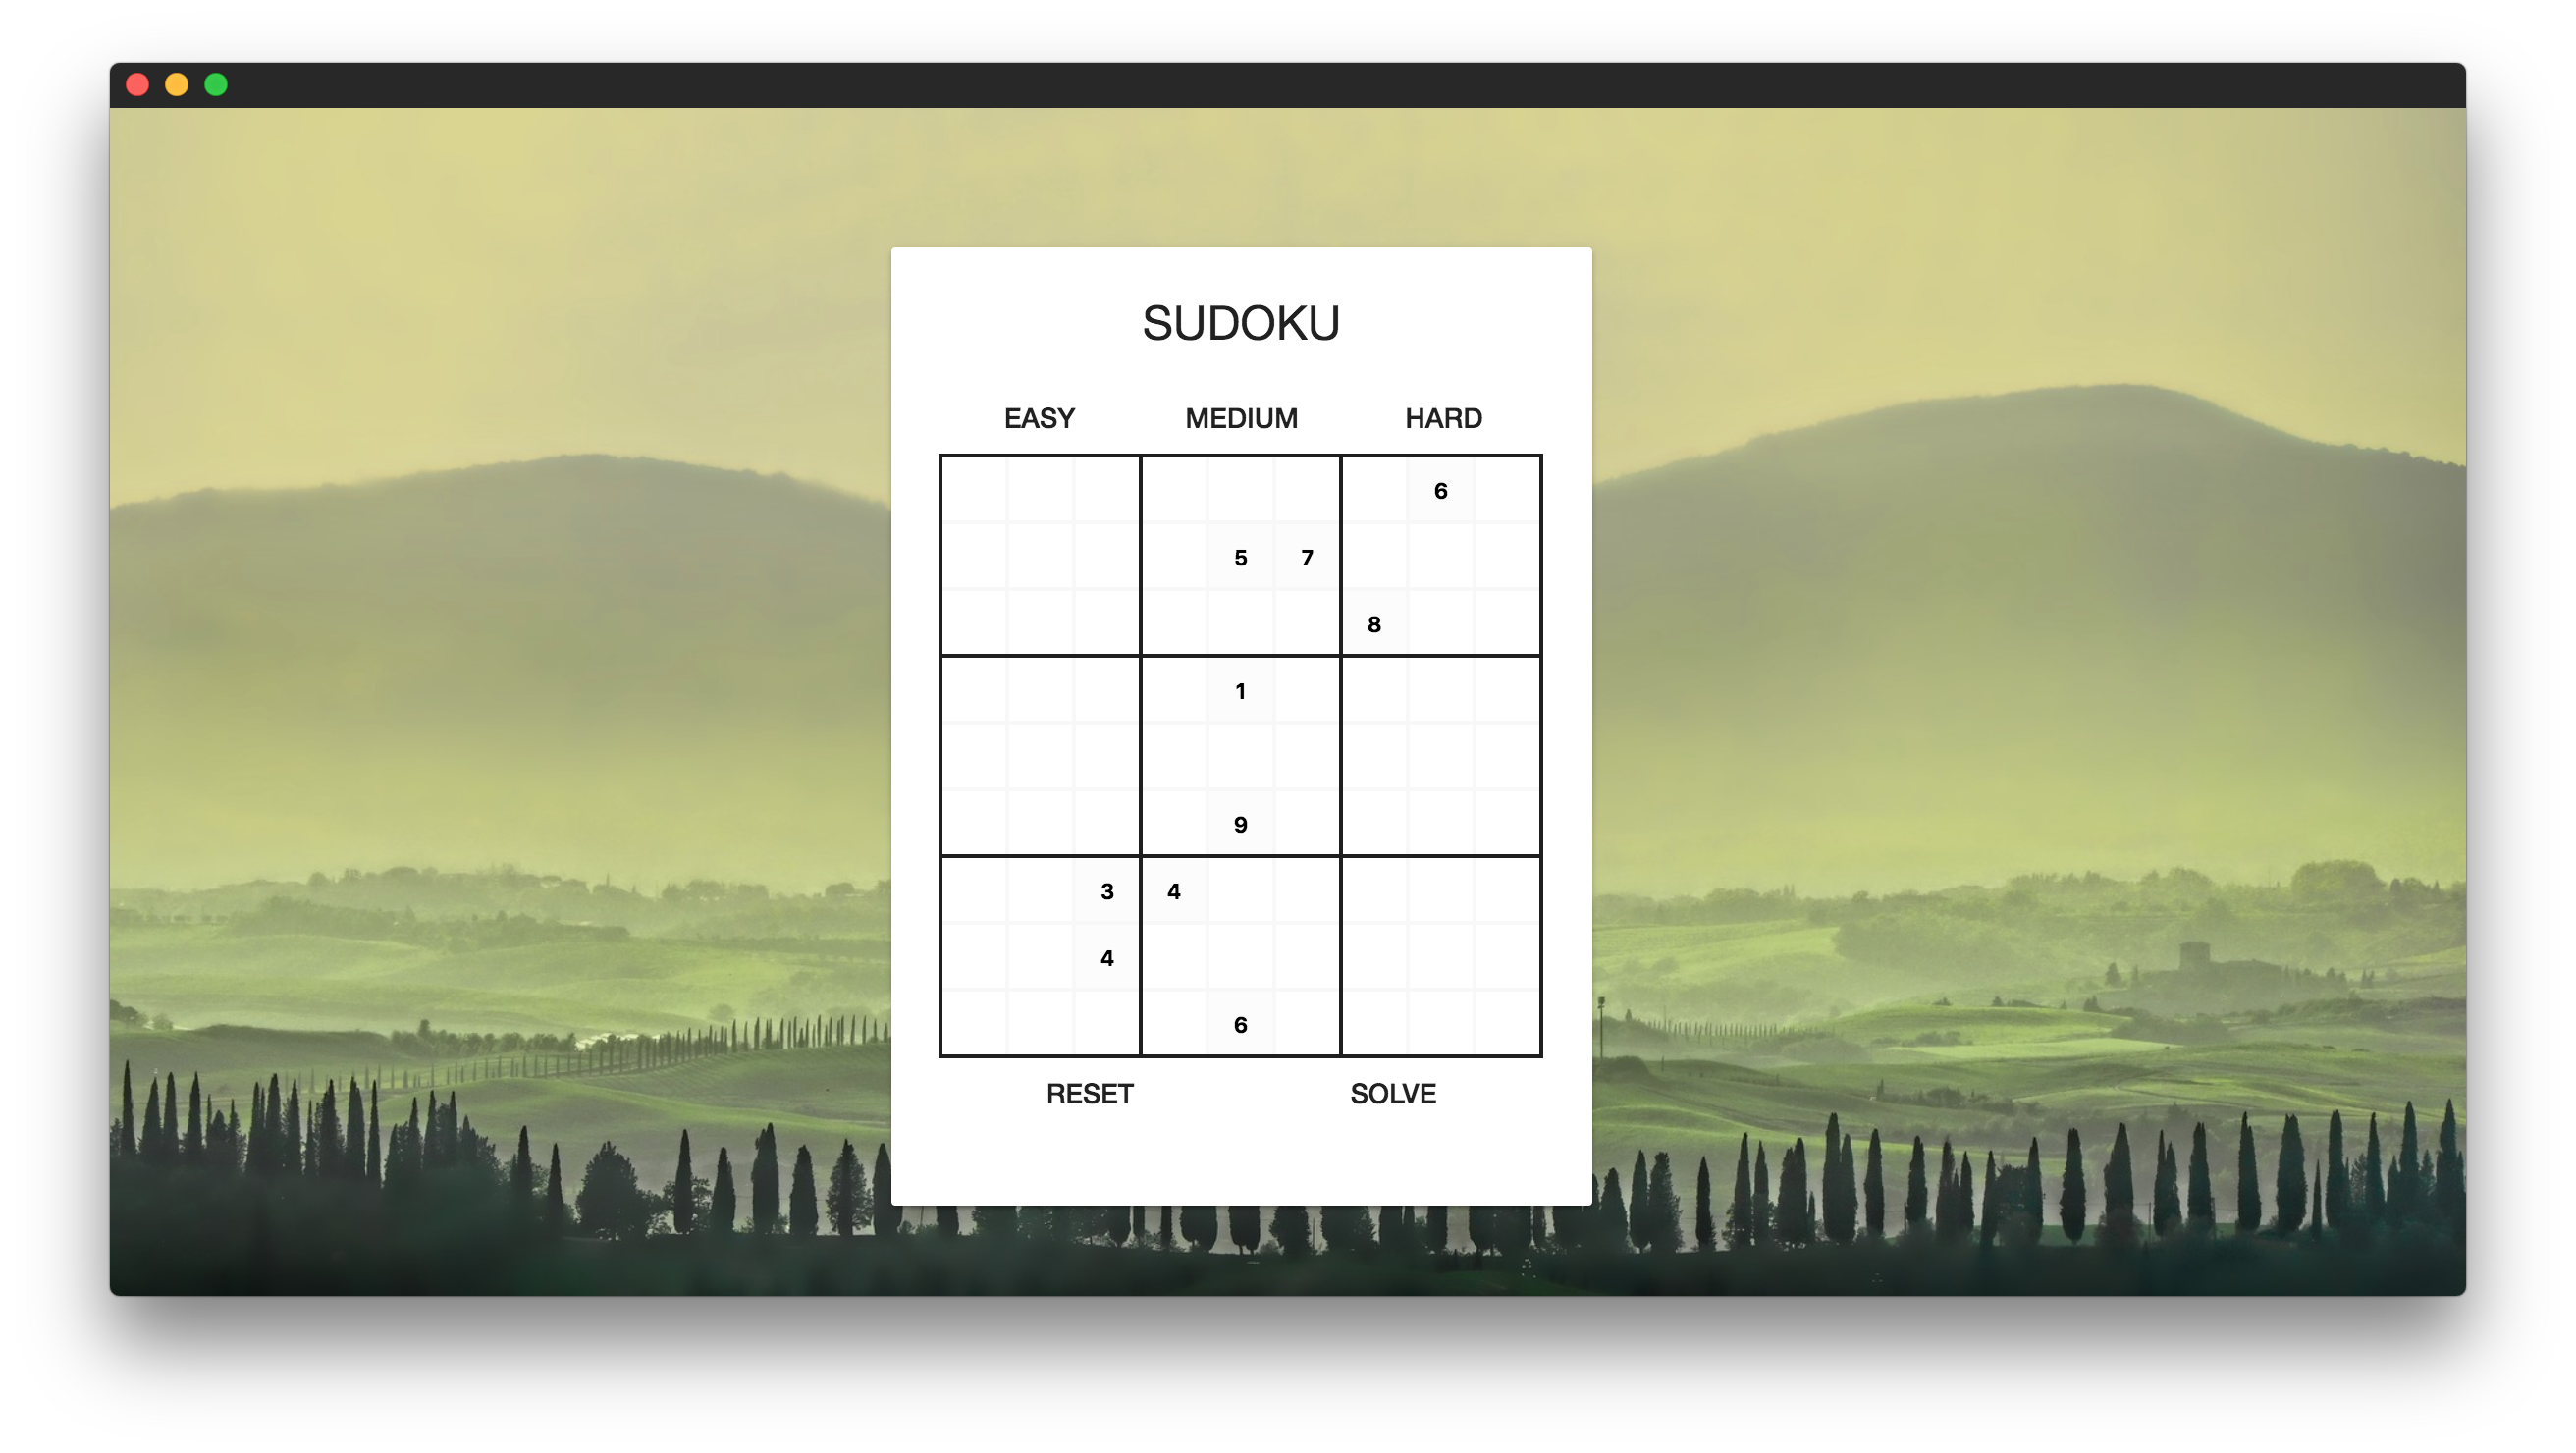
\includegraphics[width=\textwidth]{sudoku.png}
  \caption{Screenshot of the game}
\end{figure}
\par\vspace{1cm}

When the application is started, the user can choose the difficulty level, Electron then
randomly generates a sudoku board. When a board is generated, it is possible that
it has no solution. The board is then sent to the sudoku solver to check
if it has a solution. Until a board with solution is found, the application
randomly tries to generate a new board.

The application runs some simple check on the input, but also if
no number is red, it does not mean that the sudoku is correct. To check the correctedness
you have to press the solve button.
The application will warn the user if the board is not satisfiable.

\section*{How does it work}
First of all, the Electron application generates a file sudoku.in with a total of
81 lines. On every line there will be a value from 1 to 9 or the letter n, which stands
for the \texttt{null} value.
Then, Electron calls the \texttt{./sat/sudoku.py} script.
The python script then imports the data. The following image represents the function that reads the sudoku.in
file and stores the values in an array of arrays called grid.

\begin{figure}[H]
  \centering
  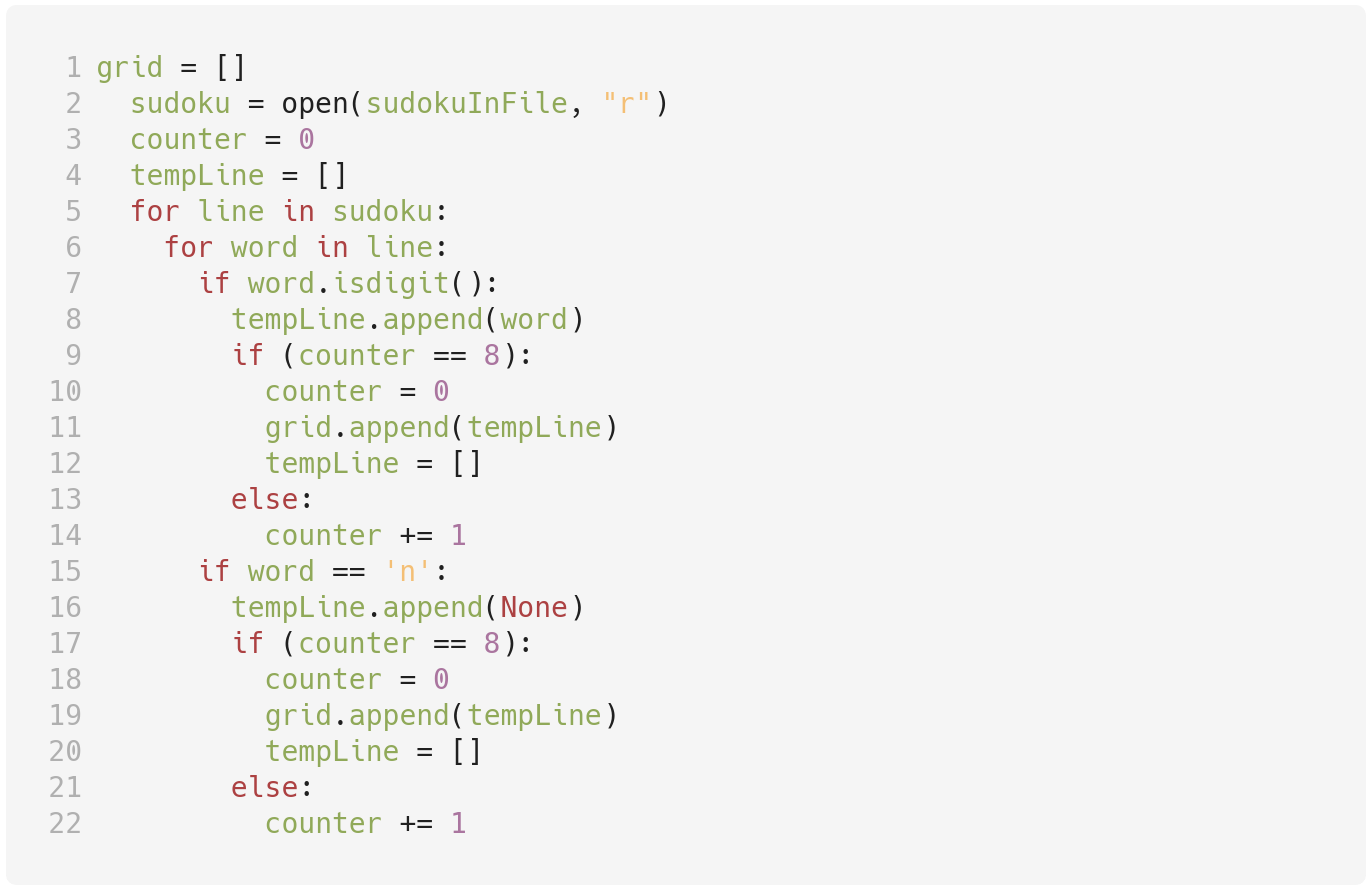
\includegraphics[width=\textwidth]{readFile.png}
  \caption{The function that imports the grid from the sudoku.in file}
\end{figure}
\clearpage

When the data is read, the next function that is run is the following:

\begin{figure}[H]
  \centering
  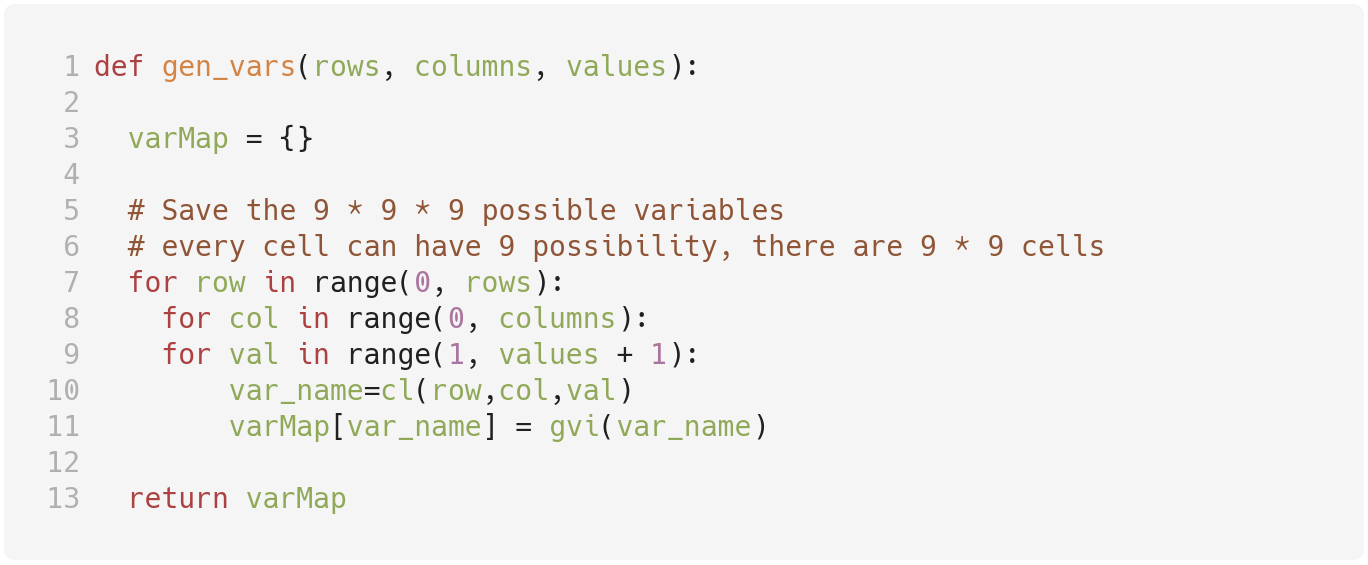
\includegraphics[width=\textwidth]{genVars.png}
  \caption{\texttt{gen\_vars} function}
\end{figure}

This function defines the variables. The idea is simple, for every
cell there can be a value from 1 to 9. This means we have \(9 \times 9 \times 9 \) different
variables, as we have \(9 \times 9 \) different cells and every single one
can contain 9 different values.
\par\vspace{0.5cm}

After this function, the script runs \texttt{genSudokuConstr()}.
This function is divided in four different parts. Each of them
adds some clauses.

\begin{figure}[H]
  \centering
  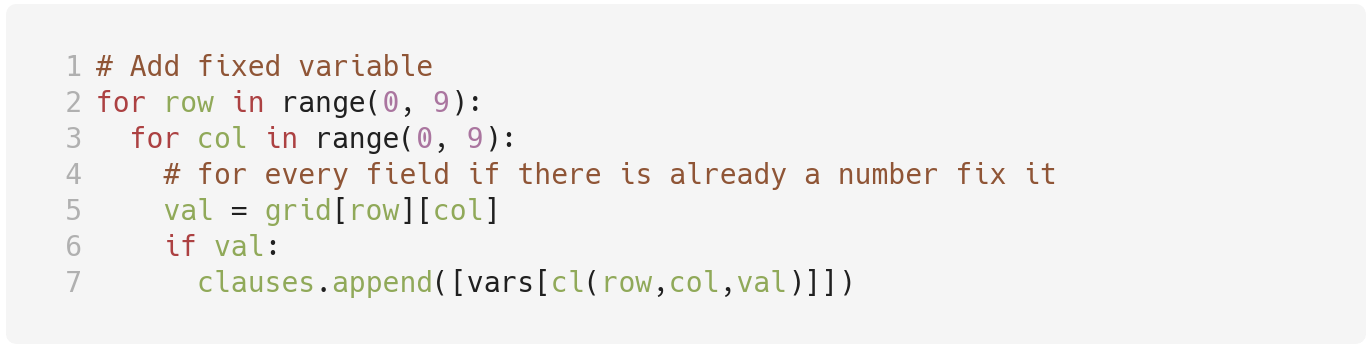
\includegraphics[width=\textwidth]{clause_01.png}
  \caption{Add clause for existing values}
\end{figure}

This part of code adds a clause for every value existing
in the grid. This means that if cell\(_{i,j}\) contains the value
7, this is added as a clause. So the SAT solver knows that in
that cell there has to be the value 7.

\begin{figure}[H]
  \centering
  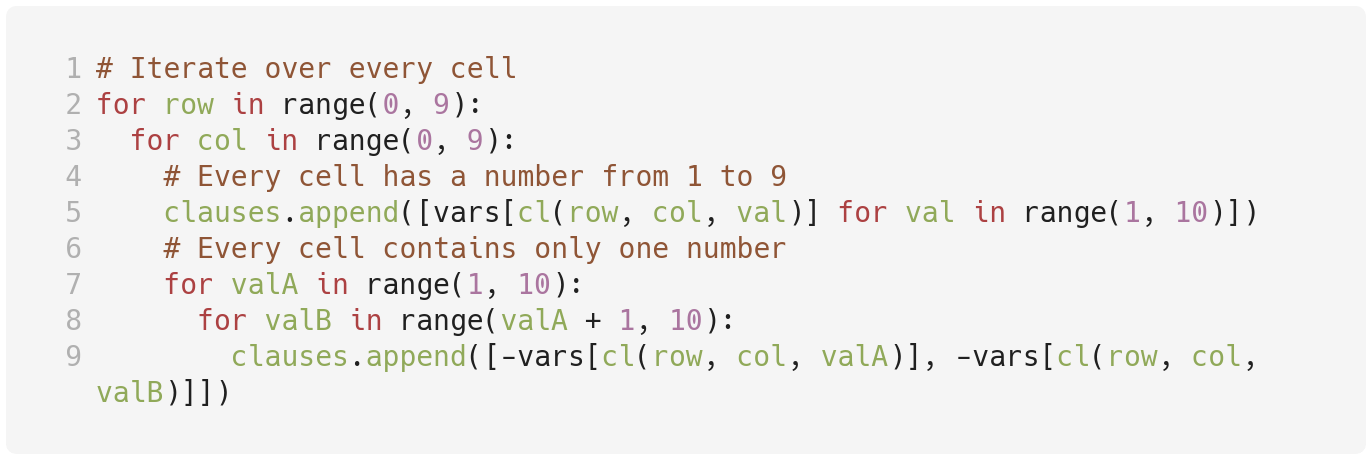
\includegraphics[width=\textwidth]{clause_02.png}
  \caption{Every cell contains a number from 1 to 9}
\end{figure}

This part of code states that in every column and every row there has to be one of the values
from 1 to 9. Starting from line 6 in states that in every
cell there can only be one possible value.

\begin{figure}[H]
  \centering
  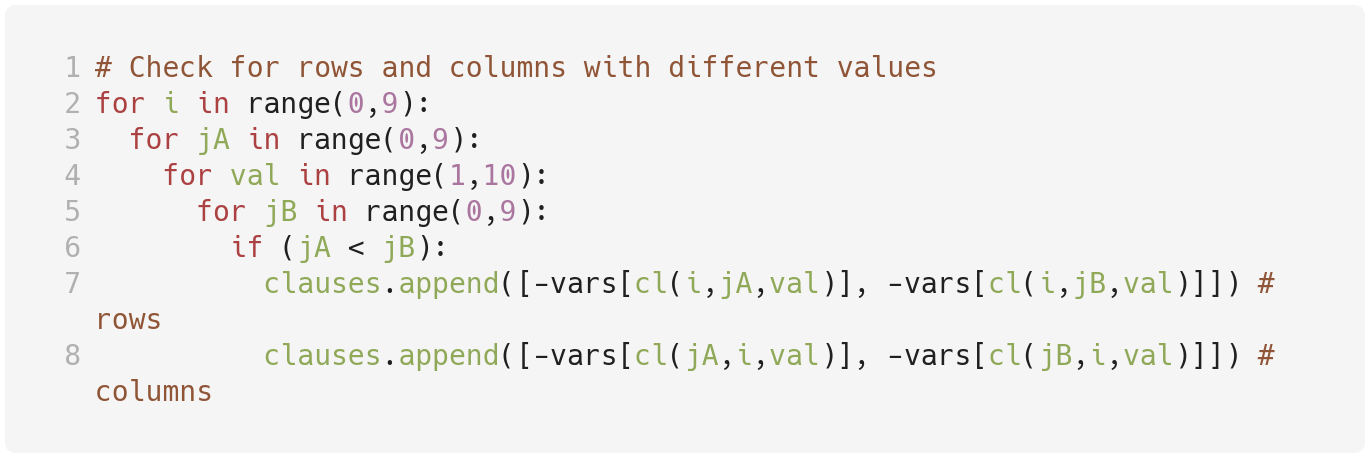
\includegraphics[width=\textwidth]{clause_03.png}
  \caption{Every column and row has different values}
\end{figure}

This part of code states that in every column and every row there
can be only one value.

\begin{figure}[H]
  \centering
  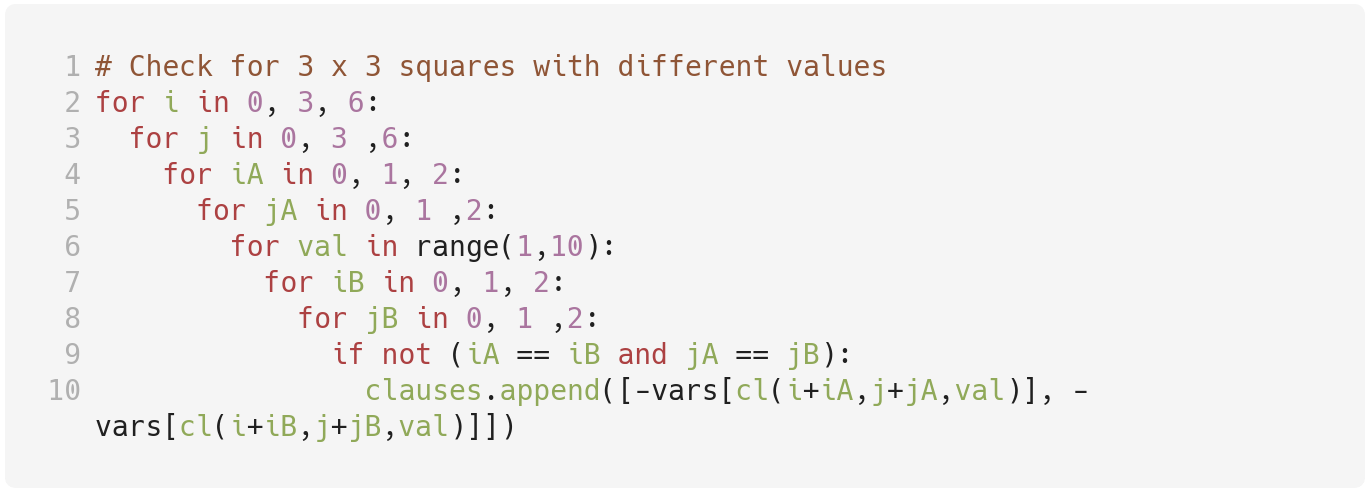
\includegraphics[width=\textwidth]{clause_04.png}
  \caption{Differente values in \(3 \times 3 \) blocks}
\end{figure}

This part of code states that in \(3 \times 3 \) block there are no
repetitions on the same number.
\par\vspace{0.5cm}

After this, the SAT solver is executed.
The grid is then written back to file and the Electron application reads it back in.
The grid is then displayed if the result is successful, otherwise a warning will be showed.

\begin{figure}[H]
  \centering
  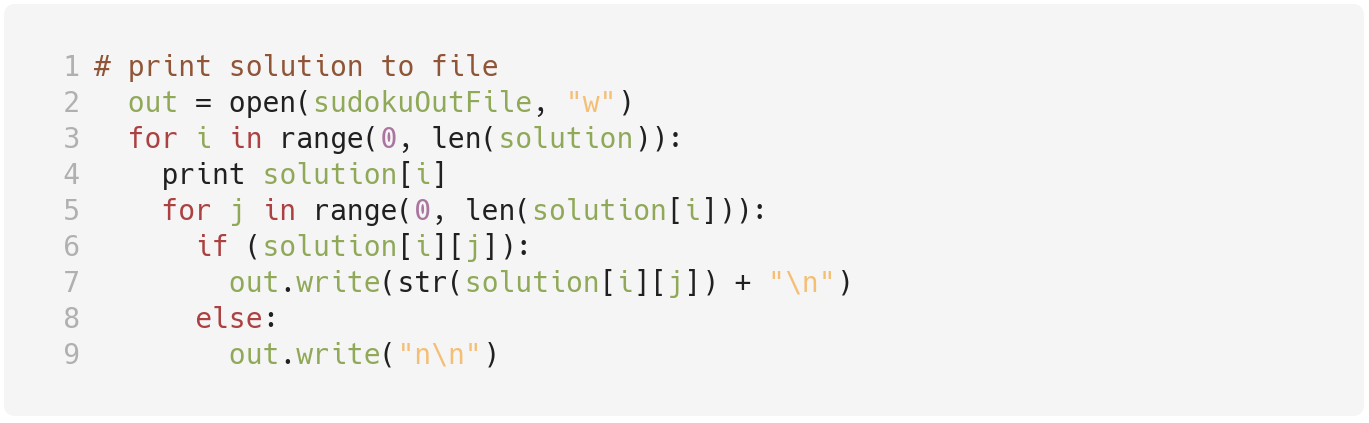
\includegraphics[width=\textwidth]{printBack.png}
  \caption{Output result to file \texttt{sudoku.out}}
\end{figure}

\section*{Encountered problems}
We did not encounter any problem as sudoku has predefined constraints,
thus it is straightforward to transform into a SAT problem.

\section*{Alternative solutions}
For the same reason as above, sudoku does not seem to have alternative solutions.

\end{document}